% \documentclass[man]{apa7}
\documentclass[stu]{apa7}

\usepackage{lipsum}

\usepackage[american]{babel}
\usepackage{multirow}
\usepackage{bm}
\usepackage{float}
\usepackage{subcaption}
\usepackage{xcolor}
\usepackage{amsmath}
\usepackage{nicematrix}
\usepackage{longtable}
\usepackage{fancyvrb}
\usepackage{listings}
\usepackage{lineno}
\usepackage{ragged2e}
\usepackage{graphicx}
\usepackage{pgfplots}
\pgfplotsset{compat=1.18}

\usepackage{xcolor} 
\colorlet{reviewColour}{blue}

\usepackage[figuresright]{rotating}

\newcommand*{\Scale}[2][4]{\scalebox{#1}{$#2$}}%
\renewcommand{\raggedright}{\justifying}

\usepackage{csquotes}
\usepackage[style=apa,sortcites=true,sorting=nyt,backend=biber,uniquename=false]{biblatex}
\DeclareLanguageMapping{american}{american-apa}
\addbibresource{references.bib}
% \DeclareLanguageMapping{english}{english-apa}
% \linenumbers

% \renewcommand{\raggedright}{\iustifying}

\hypersetup{
  colorlinks=true,
  linkcolor=blue,
  urlcolor=blue,
  citecolor=blue,
}

\title{Dichotomous Predictors and Outcomes in Multilevel Modeling: Understanding Within and Contextual Effects}
\shorttitle{DRAFT: \today}

\author{\textbf{Ward B. Eiling (s9294163)} \vspace{1cm}}
\authorsaffiliations{Department of Methodology and Statistics, Faculty of Social and Behavioural Sciences, Utrecht University \vspace{1cm}}
\course{}
\professor{prof. dr. Ellen Hamaker \& dr. Jeroen Mulder \vspace{1cm}}
\duedate{\today \vspace{1cm} \vspace{1cm}}
\note{Word count: XXXX/12,000 \\ FETC-approved: 24-2003 \\ \vspace{1cm} \textit{Candidate Journal: Psychological Methods}}

% \leftheader{Weiss}

% \abstract{INSERT ABSTRACT.}

% \keywords{APA style, demonstration}

% \authornote{
%    \addORCIDlink{Daniel A. Weiss}{0000-0000-0000-0000}

%   Correspondence concerning this article should be addressed to Daniel A. Weiss, Department of Educational Psychology, Counseling and
%   Special Education, A University Somewhere, 123 Main St., Oneonta, NY
%   13820.  E-mail: daniel.weiss.led@gmail.com}

\begin{document}

\maketitle

% Start the manuscript

% \subsection{Paragraph 1: Set the stage}

Across a wide range of disciplines, researchers analyze clustered longitudinal data to investigate prospective causal relationships between variables. When analyzing such data, psychological researchers commonly use the multilevel modeling framework \parencite[MLM,][]{bauer_fitting_2011}. A fundamental concern within the MLM literature is that the relationship between a predictor and an outcome may differ across levels of analysis \parencite[e.g.,][]{enders_centering_2007, kreft_effect_1995, raudenbush_hierarchical_2002}. In the context of longitudinal data, this implies that relationships across time captured at the within-person level of a model may differ from stable, between-person relationships as captured at the between-person level of a model. This discrepancy, known as the \textit{contextual effect}, is particularly important because failing to account for it results in an ``uninterpretable blend'' of within- and between-cluster relationships \parencite[139]{raudenbush_hierarchical_2002}. This blending obscures the within-person effect, which is typically the target for causal interpretation.

% \subsection{Paragraph 2: Build up the tension}

The centering of predictor and outcome variables is a common approach to separate within-person effects from between-person effects. There exist multiple centering strategies and each has important consequences for the estimation and interpretation of parameter estimates. However, most research focuses on continuous predictors, with relatively little guidance on how to distinguish within- and between-cluster differences for dichotomous predictors \parencite[for brief treatments, see][]{yaremych_centering_2023, enders_centering_2007, raudenbush_hierarchical_2002}. Given this limited coverage, it is unsurprising that applied researchers often rely on intuition or avoid centering altogether when specifying categorical predictors \parencite{yaremych_centering_2023}. It is even less clear how to think about within- and between-person effects in the context of multilevel models with a dichotomous \textit{outcome} \parencite[However, see][]{austin_intermediate_2017, bolger_modeling_2013}. This gap in methodological guidance is concerning since categorical variables are ubiquitous within the social sciences and researchers may be left unaware of how to specify their models correctly. 

% \subsection{Paragraph 3: Build up the tension even more}

In biostatistics and related fields, researchers often prefer Generalized Estimating Equations (GEE) for analyzing clustered data with dichotomous outcomes, primarily due to its fewer assumptions compared to random-effects models \parencite[]{mcneish_unnecessary_2017}. GEE provides a general framework for modeling dependent data without explicitly incorporating random effects, instead requiring the user to specify a working correlation structure \parencite{zeger_models_1988}. Common choices include an exchangeable structure, which assumes a constant correlation among all within-cluster observations, or an independence structure, which assumes no within-cluster dependence. As GEE gains traction in psychology \parencite[]{mcneish_unnecessary_2017}, researchers familiar with multilevel modeling may question how GEE compares to multilevel models, specifically whether the debate about separating within- from between-person effects using a centering strategy also applies when a GEE modeling approach is taken. In addition, it may be wondered what effects GEE estimates and how this depends upon the user specified working correlation structure.

% \subsection{Paragraph 4: Aim of the Current Study (potential resolve?)}

The goals of this paper are twofold. First, we aim to determine how we should think about within and between effects with a dichotomous X and/or Y. Second, we study the degree to which we can correctly estimate these effects with multilevel model and GEE implementations. Using simulations, we will study the performance of estimates of within-person effects across (a) a multilevel modeling versus a GEE modeling approach; (b) different centering strategies; (c) different measurement levels (continuous and dichotomous) of the predictor and the outcome; and (d) sample sizes, both at the cluster-level as well as within-cluster. We will compare the performance of different methods in terms of bias and coverage rates. Based on the simulations, we will shed light on potential concerns that may endanger the correct interpretation of results. By doing this, we guide researchers with correctly specifying models and interpret the parameter estimates in the context of dichotomous predictors an outcomes.

% \subsection{Paragraph 6: Outline current paper}

This article is organized as follows. In the first section we elaborate on the four data generating models to conceptualize within- and between-person effects in the context of varying measurement levels of predictor and outcome. For didactical reasons, we accompany the equations with a running example. In the second section, we discuss different modeling approaches and ways of centering. In the third section, we perform a simulation study to show how the data generating models can be estimated with these modeling approaches. Finally, we summarize the main findings, discuss limitations and promising avenues for future research.

% \begin{center}
%     \captionof{table}{Cross-Table Scenarios}
%     \label{tab:crosstable}
    
%     \begin{tabular}{l l l l } \toprule
%  &  & \multicolumn{2}{c}{Outcome} \\
%  &  & Continuous & Dichotomous \\ 
%  \hline
% \multirow{2}{*}{Predictor} & Continuous &  Known& ?\\ 
%  & Dichotomous &  ?&  ?\\
% \bottomrule
% \end{tabular}
% \end{center}

\section{Running Empirical Example}

To illustrate within- and between-person effects, we use a running example grounded in prior empirical work on the effect of mindfulness (\(X_{it}\)) on anger (\(Y_{it}\)). Numerous studies have shown that, across individuals, those with higher trait mindfulness report lower levels of aggressiveness \parencite[]{brown_benefits_2003, borders_could_2010, kashdan_what_2016, baer_relationships_2011, eisenlohr-moul_both_2016}. Mindfulness also shows substantial within-person variability over time \parencite[]{brown_benefits_2003, kiken_state_2015}, and evidence suggests that on days when individuals report higher-than-usual mindfulness, they also report lower levels of state anger \parencite[]{eisenlohr-moul_both_2016}. Both within- and between-person associations are typically negative, though effect sizes depend on the specific operationalization \parencite{eisenlohr-moul_both_2016}. Nevertheless, between-person associations tend to be larger, consistent with trait mindfulness being a more stable and robust predictor of anger-related outcomes than day-to-day fluctuations.

In our example dataset, participants report their momentary (``right now'') states each evening. In the binary predictor condition, mindfulness is coded as 1 if the participant practiced mindfulness that day and 0 otherwise. In the continuous predictor condition, it reflects self-reported mindfulness that day, assessed by the reverse-scored acting with awareness item ``I found myself doing things without paying attention to them,'' rated from 1 (never or very rarely true) to 5 (very often or always true) \parencite[]{baer_using_2006}. The outcome variable, anger, is operationalized in two parallel ways. In the binary condition, participants report whether they had an inclination to express anger, based on the item “If people were annoying me today, I would tell them what I think of them” (1 = yes, 0 = no) \parencite[]{buss_aggression_1992}. In the continuous condition, anger intensity is captured by the PANAS item ``Indicate to what degree you feel hostile right now,'' rated from 0 (very slightly or not at all) to 5 (extremely) \parencite[]{watson_panas-x_1994}.

\section{Data Generating Models}

In this section we introduce the four data generating models (DGMs) that are used in the simulation study. For description of these models, We follow the common multilevel notation of \textcite{raudenbush_hierarchical_2002}. The DGMs differ in the measurement level of the predictor $X$ and the outcome $Y$ (see Figure~\ref{fig:path2}). In all four DGMs we generate a single level 1 predictor $X_{it}$ such that there are stable individual (between-person) differences in the mean levels of $X$ per individual $i$, as well as within-person variation across timepoints $t$. In addition, the DGMs comprise person-specific unobserved heterogeneity in the baseline levels on outcome $Y$, represented by $u_{0i}$. 

% For illustrative purposes, we use a running example based on an empirical studies, centered on the effect of mindfulness (\(X_{it}\)) on anger (\(Y_{it}\)). Previous studies have found that trait-level between-person differences in mindfulness predict aggressiveness \parencite[]{brown_benefits_2003, borders_could_2010, kashdan_what_2016, baer_relationships_2011, eisenlohr-moul_both_2016}. In addition to stable individual differences, mindfulness facets also demonstrate significant state-level, within-person variability \parencite[]{kiken_state_2015, brown_benefits_2003, eisenlohr-moul_weekly_2016, eisenlohr-moul_both_2016}. In the data we generate, we assume that each evening, a person reports his or her momentary ("right now") states. In the binary predictor condition, the variable indicates whether or not the person practiced mindfulness on a given day; in the continuous condition, it reflects the degree to which they felt mindful that day captured by the item ``I found myself doing things without paying attention to them'' \parencite[reverse scored, ]{baer_using_2006}. The outcome variable is similarly operationalized: in the binary case, it captures whether the individual had an inclination to express anger captured by the item ``If people were annoying me today, I would tell them what I think of them'' \parencite[]{buss_aggression_1992} rated 1 if yes and 0 if no; in the continuous case, it reflects the daily anger itensity captured by the PANAS item "Indicate to what degree you feel hostile right now" rated on a scale from 0 (very slightly or not at all today) to 5 (extremely today) \parencite[]{watson_panas-x_1994}.


% Models were parametrized as Mundlak's contextual model \parencite[]{mundlak_pooling_1978}, implying they include an uncentered predictor and cluster mean as predictors.

% \begin{itemize}
%     \item continuous predictor: sleep problems
%     \item continuous outcome: anxiety
%     \item dichotomous predictor: mindfulness practice
%     \item dichotomous outcome: interpersonal conflict
% \end{itemize}

\begin{center}
    \captionof{figure}{Path diagrams of Generative Models with Within-Person ($\beta_1$) and Contextual Effect ($\gamma_{01}$)}
    % Top row
    \begin{minipage}[t]{.49\linewidth}
        \centering
        \begin{subfigure}[b]{\linewidth}
            \centering
            
\includegraphics[height=6.5cm]{Figures/pathdiagrams-cropped-contxy.drawio.pdf}
            \caption{Continuous X and Y}\label{fig:path-contxy}
        \end{subfigure}
    \end{minipage}
    \hfill
    \begin{minipage}[t]{.49\linewidth}
        \centering
        \begin{subfigure}[b]{\linewidth}
            \centering
            
\includegraphics[height=6.5cm]{Figures/pathdiagrams-cropped-binxconty.drawio.pdf}
            \caption{Binary X and Continuous Y}\label{fig:path-binxconty}
        \end{subfigure}
    \end{minipage}

    % \vskip 1em

    % Bottom row
    \begin{minipage}[t]{.49\linewidth}
        \centering
        \begin{subfigure}[b]{\linewidth}
            \centering
            
\includegraphics[height=7.5cm]{Figures/pathdiagrams-cropped-contxbiny.drawio.pdf}
            \caption{Continuous X and Binary Y}\label{fig:path-contxbiny}
        \end{subfigure}
    \end{minipage}
    \hfill
    \begin{minipage}[t]{.49\linewidth}
        \centering
        \begin{subfigure}[b]{\linewidth}
            \centering
            
\includegraphics[height=7.5cm]{Figures/pathdiagrams-cropped-binxy.drawio.pdf}
            \caption{Binary X and Y}\label{fig:path-binxy}
        \end{subfigure}
    \end{minipage}
    \vspace{-0.5cm}
    \label{fig:path}
    \begin{flushleft}
    \begin{figurenote}
    Path diagrams of the four data-generating models, varying by predictor type $X$ (columns) and outcome type $Y$ (rows), each either continuous or binary. In all models, the outcome is regressed on the predictor, and the person-level predictor mean $\mu_X$ predicts the outcome intercept $\beta_0$, yielding a within-person slope $\beta_1$ and a contextual effect $\gamma_{01}$. Circles represent latent variables, squares observed variables. Solid arrows denote linear relations; dotted arrows indicate logit transformations (\texttt{plogis} in \texttt{R}); dashed arrows indicate Bernoulli sampling with probability $\pi$ (\texttt{rbinom} in \texttt{R}).
    
    % Path diagrams of four data generating models that vary in predictor type $X$ (column wise) and outcome type $Y$ (row wise), both of which are either continuous or binary. Models are based regressing the outcome variable on the predictor, while using the latent mean per person on the predictor $\mu_X$ to predict the intercept $\beta_{0}$ of the outcome. This results in the within-person slope $\beta_1$ and the contextual effect $\gamma_{01}$. Circles denote latent variables, squares denote observed variables, and arrows represent relationships. Solid arrows indicate linear associations, dotted arrows represent logit transformations (\texttt{plogis} in \texttt{R}), and dashed arrows indicate Bernoulli sampling with probability $\pi$ (\texttt{rbinom} in \texttt{R}).
    % Circles represent latent variables, squares represent observed variables, and arrows indicate relationships. Solid arrows denote linear associations, with a coefficient of 1 indicating a one-to-one relationship. Dotted arrows represent logit transformations (\texttt{plogis} in \texttt{R}), and dashed arrows represent Bernoulli sampling based on the probability $\pi$ (\texttt{rbinom} in \texttt{R}).
    \end{figurenote}
    \end{flushleft}
\end{center}

% \begin{center}
%     \captionof{figure}{Path diagrams of Generative Models with Within-Person ($\beta_1$) and Contextual Effect ($\gamma_{01}$)}
%     % Top row
%     \begin{minipage}[t]{.49\linewidth}
%         \centering
%         \begin{subfigure}[b]{\linewidth}
%             \centering
%             
\includegraphics[width=\linewidth, height=8cm, keepaspectratio]{Figures/pathdiagrams-contxy.drawio.pdf}
%             \caption{Continuous X and Y}\label{fig:path-contxy}
%         \end{subfigure}
%     \end{minipage}
%     \hfill
%     \begin{minipage}[t]{.49\linewidth}
%         \centering
%         \begin{subfigure}[b]{\linewidth}
%             \centering
%             
\includegraphics[width=\linewidth, height=8cm, keepaspectratio]{Figures/pathdiagrams-contxbiny.drawio.pdf}
%             \caption{Continuous X and Binary Y}\label{fig:path-contxbiny}
%         \end{subfigure}
%     \end{minipage}

%     % \vskip 1em

%     % Bottom row
%     \begin{minipage}[t]{.49\linewidth}
%         \centering
%         \begin{subfigure}[b]{\linewidth}
%             \centering
%             
\includegraphics[width=\linewidth, height=8cm, keepaspectratio]{Figures/pathdiagrams-binxconty.drawio.pdf}
%             \caption{Binary X and Continuous Y}\label{fig:path-binxconty}
%         \end{subfigure}
%     \end{minipage}
%     \hfill
%     \begin{minipage}[t]{.49\linewidth}
%         \centering
%         \begin{subfigure}[b]{\linewidth}
%             \centering
%             
\includegraphics[width=\linewidth, height=8cm, keepaspectratio]{Figures/pathdiagrams-binxy.drawio.pdf}
%             \caption{Binary X and Y}\label{fig:path-binxy}
%         \end{subfigure}
%     \end{minipage}
%     \vspace{-1cm}
%     \label{fig:path}
%     \begin{flushleft}
%     \begin{figurenote}
%     Circles represent latent variables, squares represent observed variables, and arrows indicate relationships. Solid arrows denote linear associations, with a coefficient of 1 indicating a one-to-one relationship. Dotted arrows represent logit transformations (\texttt{plogis} in \texttt{R}), and dashed arrows represent Bernoulli sampling based on the probability $\pi$ (\texttt{rbinom} in \texttt{R}).
%     \end{figurenote}
%     \end{flushleft}
% \end{center}

% \begin{center}
% \captionof{figure}{Path diagrams of Generative Models with Within-Person ($\beta_\text{w}$) and Contextual Effect ($\gamma_{01}$)}

% \begin{minipage}[t]{.49\linewidth}
%     \centering
%     \begin{subfigure}[b]{\linewidth}
%         \centering
%         
\includegraphics[width=\linewidth, height=8cm, keepaspectratio]{Figures/pathdiagrams-contxy.drawio.pdf}
%         \caption{Continuous X and Y}\label{fig:path-contxy}
%     \end{subfigure}
%     \vspace{1em}
%     \begin{subfigure}[b]{\linewidth}
%         \centering
%         
\includegraphics[width=\linewidth, height=8cm, keepaspectratio]{Figures/pathdiagrams-binxconty.drawio.pdf}
%         \caption{Binary X and Continuous Y}\label{fig:path-binxconty}
%     \end{subfigure}
% \end{minipage}
% \hfill
% \begin{minipage}[t]{.49\linewidth}
%     \centering
%     \begin{subfigure}[b]{\linewidth}
%         \centering
%         
\includegraphics[width=\linewidth, height=8cm, keepaspectratio]{Figures/pathdiagrams-contxbiny.drawio.pdf}
%         \caption{Continuous X and Binary Y}\label{fig:path-contxbiny}
%     \end{subfigure}
%     \vspace{1em}
%     \begin{subfigure}[b]{\linewidth}
%         \centering
%         
\includegraphics[width=\linewidth, height=8cm, keepaspectratio]{Figures/pathdiagrams-binxy.drawio.pdf}
%         \caption{Binary X and Y}\label{fig:path-binxy}
%     \end{subfigure}
% \end{minipage}

% \vspace{-0.5cm}
% \label{fig:path}

% \begin{flushleft}
% \begin{figurenote}
% Circles represent latent variables, squares represent observed variables, and arrows indicate relationships. Solid arrows denote linear associations, with a coefficient of 1 indicating a one-to-one relationship. Dotted arrows represent logit transformations (\texttt{plogis} in \texttt{R}), and dashed arrows represent Bernoulli sampling based on the probability $\pi$ (\texttt{rbinom} in \texttt{R}).
% \end{figurenote}
% \end{flushleft}
% \end{center}


\subsection{DGM 1: Continuous Predictor and Outcome}

To illustrate the DGM for a continuous predictor and outcome, we consider the case of how mindfulness, operationalized as acting with awareness, relates to daily experiences of anger. We begin by generating person-level heterogeneity in mindfulness. Individuals differ in their general tendency to act with awareness, which we represent by a person-specific latent mean \( \mu_{X,i} \). This stable component is drawn from a normal distribution:
\begin{equation}
    \label{eqn:xbetweencontxy}
    \mu_{X,i} \sim \mathcal{N}(0, \sigma^2_{X,\text{b}}),
\end{equation}
where \( \sigma^2_{X,\text{b}} \) captures between-person variability. Next, we model intraindividual fluctuations in mindfulness across measurement occasions. These within-person deviations are drawn from:
\begin{align}
    \label{eqn:xwithincontxy}
    X_{w,it} &\sim \mathcal{N}(0, \sigma^2_{X,\text{w}}), \\
    \label{eqn:relationwithinmundlak}
    X_{it} &= \mu_{X,i} + X_{w,it},
\end{align}
where \( X_{it} \) is the observed mindfulness score for person \( i \) at time \( t \), composed of the person’s stable tendency \( \mu_{X,i} \) and their momentary deviation \( X_{w,it} \). We then model daily anger (\( Y_{it} \)) as a function of both levels of mindfulness. At the within-person level, we specify:
\begin{equation}
    \label{eqn:yit-generationmlm}
    Y_{it} = \beta_{0i} + \beta_{1} X_{it} + e_{it},
\end{equation}
where \( \beta_{0i} \) is an individual-specific intercept capturing baseline anger, \( \beta_1 \) is the fixed \textit{within-person effect} of mindfulness on anger, and \( e_{it} \sim \mathcal{N}(0, \sigma^2_e) \) is a time-specific residual. To introduce between-person effects, the individual-specific intercept \( \beta_{0i} \) is modeled as a function of the person’s average mindfulness:
\begin{equation}
    \label{eqn:beta0-generationcontxy}
    \beta_{0i} = \gamma_{00} + \gamma_{01} \mu_{X,i} + u_{0i},
\end{equation}
where \( \gamma_{00} \) is the grand mean of anger, \( \gamma_{01} \) is the contextual effect of trait mindfulness on anger, and \( u_{0i} \sim \mathcal{N}(0, \sigma^2_u) \) is a person-specific residual representing unobserved heterogeneity in baseline anger not explained by mindfulness. A large \( \sigma^2_u \) suggests that trait mindfulness only partially accounts for stable individual differences in anger. Substituting the between-person model into the within-person equation yields the full generative model:
\begin{equation}
    Y_{it} = \gamma_{00} + \gamma_{01} \mu_{X,i} + u_{0i} + \beta_1 X_{it} + e_{it}.
\end{equation}
This formulation decomposes the total effect of mindfulness on anger into within- and between-person components. The coefficient \( \beta_1 \) captures the within-person effect (i.e., the extent to which anger changes when an individual is more or less mindful than usual), while the \textit{contextual effect} \( \gamma_{01} \) captures the degree to which the between-person effect---the association between a person's typical mindfulness level (\( \mu_{X,i} \)) and stable anger level---differs from the within-person effect. The implied between-person effect is then given by $\beta_\text{b} = \gamma_{01} + \beta_1$ \parencite{mundlak_pooling_1978}. A positive \( \gamma_{01} \) implies that individuals who are more mindful on average experience more anger than would be expected based only on the within-person relationship. A negative \( \gamma_{01} \) implies that individuals who are more mindful on average experience less anger than would be expected based solely on the within-person relationship—suggesting a trait-level benefit of mindfulness. 

Empirical studies often find that between-person associations are larger in magnitude than within-person associations, implying the presence of a \textit{negative} contextual effect. To reflect this, we might specify the following parameter values $
\gamma_{00} = 4.5,\quad \gamma_{01} = -0.6,\quad \beta_1 = -0.4$ so that $\beta_\text{b} = -0.6 - 0.4 = 1$. As visualized in Figure~\ref{fig:withinbetween-contxy}, these parameters yield a stronger negative association at the between-person level than at the within-person level.

\begin{center}
    \captionof{figure}{Within- and Between-Person Effects of Continuous Predictor and Outcome}

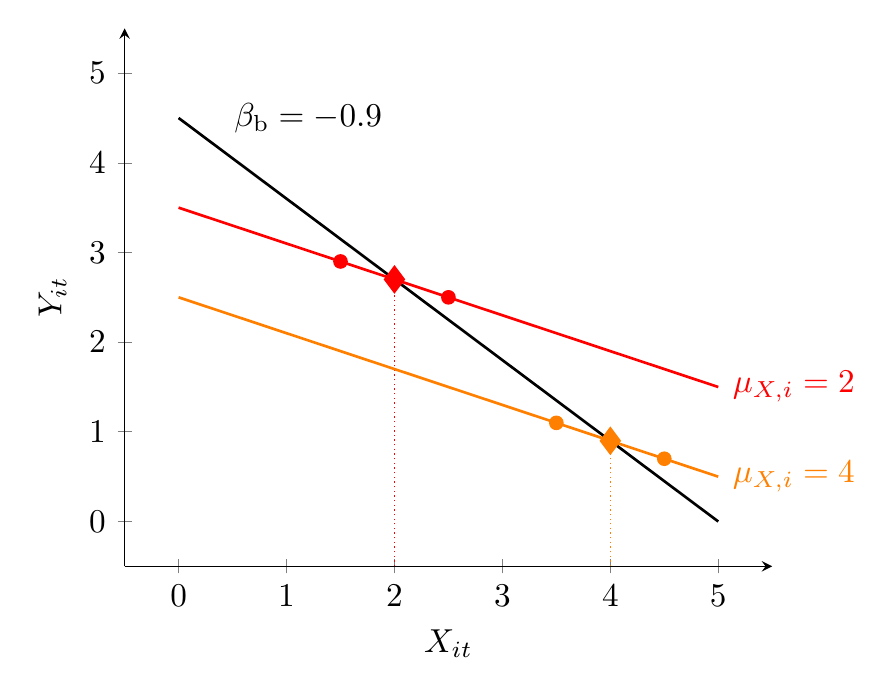
\begin{tikzpicture}[scale=1.2]
    \begin{axis}[
        axis x line=left, 
        axis y line=left, 
        xlabel={$X_{it}$}, ylabel={$Y_{it}$},
        xmin=0, xmax=5, ymin=0, ymax=5,
        xtick={0,1,2,3,4,5},
        ytick={0,1,2,3,4,5},
        enlargelimits=true,
        clip=false,
        xshift=-15mm
    ]

    \pgfmathsetmacro{\gammaZero}{4.5}
    \pgfmathsetmacro{\gammaOne}{-0.5}
    \pgfmathsetmacro{\betaOne}{-0.4}
    \pgfmathsetmacro{\betaB}{-0.9}  % gamma01 + beta1

    % === Within-person: mu_X = 2 ===
    \addplot[domain=0:5, thick, red] {\gammaZero + \gammaOne*2 + \betaOne*x};
    \addplot[only marks, red] coordinates {
        (1.5, {4.5 - 0.5*2 - 0.4*1.5})
        % (2.0, {4.5 - 0.5*2 - 0.4*2.0})
        (2.5, {4.5 - 0.5*2 - 0.4*2.5})
    };
    \addplot[only marks, mark=diamond*, mark size=4pt, red] coordinates {
        (2.0, {4.5 - 0.5*2 - 0.4*2.0})
    };
    \addplot[densely dotted, thin, red] coordinates {
        (2.0, -0.5)
        (2.0, {4.5 - 0.5*2 - 0.4*2.0})
    };

    % === Within-person: mu_X = 4 ===
    \addplot[domain=0:5, thick, orange] {\gammaZero + \gammaOne*4 + \betaOne*x};
    \addplot[only marks, orange] coordinates {
        (3.5, {4.5 - 0.5*4 - 0.4*3.5})
        % (4.0, {4.5 - 0.5*4 - 0.4*4.0})
        (4.5, {4.5 - 0.5*4 - 0.4*4.5})
    };
    \addplot[only marks, mark=diamond*, mark size=4pt, orange] coordinates {
        (4.0, {4.5 - 0.5*4 - 0.4*4.0})
    };
    \addplot[densely dotted, thin, orange] coordinates {
        (4.0, -0.5)
        (4.0, {4.5 - 0.5*4 - 0.4*4.0})
    };

    % === Between-person regression line ===
    \addplot[thick, black, domain=0:5] {\gammaZero + \betaB*x};

    % === Labels ===
    \node[red] at (axis cs:5.7,1.5) {$\mu_{X,i}=2$};
    \node[orange] at (axis cs:5.7,0.5) {$\mu_{X,i}=4$};
    \node[black] at (axis cs:1.2,4.5) {$\beta_\text{b} = -0.9$};

    \end{axis}
\end{tikzpicture}

    \label{fig:withinbetween-contxy}
    \begin{figurenote}
        The solid black slope represents the between-person effect and the colored slopes the within-cluster effects. The X-axis simultaneously represents $X_{it}$ for the within-slope and $\mu_{X,i}$ for the between-slope; and the Y-axis represents $Y_{it}$ for the within slope and $Y_i$ for the between-slope. Dots reflect possible datapoints and diamonds reflect the position of $\mu_{X,i}$ on the within-person slope.
    \end{figurenote}
\end{center}

\subsection{DGM 2: Dichotomous Predictor and Continuous Outcome}

The data-generating process for a MLM with a continuous predictor is illustrated in Figure~\ref{fig:dichxconty}. Suppose we are interested in how engaging in mindfulness practice on a given day (\(X_{it}\)), coded as 1 if practiced and 0 otherwise, relates to self-reported anxiety levels (\(Y_{it}\)). Compared to an MLM with continuous predictor, introducing a dichotomous predictor modifies only the between-person equation, while the within-person equation remains unchanged (compare Figures~\ref{fig:contxy} and~\ref{fig:dichxconty}). The between-person equation now takes the form:  
\begin{equation}
    \label{eqn:beta0-generationdichxconty}
\beta_{0i} = \gamma_{00} + \gamma_{01} \pi_{Xi} + u_{0i},
\end{equation}
where \( \pi_{Xi} \) replaces the continuous cluster mean \( \mu_{X,i} \) and represents the probability of \( X_{it} = 1 \) for cluster \( i \). The composite model then becomes:
\begin{equation}
Y_{it} = \gamma_{00} + \gamma_{01} \pi_{Xi} + u_{0i} + \beta_1 X_{it} + e_{it}.
\end{equation}

% Because the predictor is now dichotomous, the interpretation of fixed effects shifts. The intercept \( \gamma_{00} \) represents the expected anxiety level for an individual with an average event probability of zero (i.e., someone who never engages in mindfulness). The within-person effect \( \beta_1 \) quantifies how an individual’s anxiety changes on days when they engage in mindfulness practice versus days when they do not. The contextual effect \( \gamma_{01} \) captures the degree to which the between-person effect---the association between a person's long-term tendency to engage in mindfulness \( \pi_{Xi} \) and their overall anxiety level---differs from the within-person effect. The between-person effect $\beta_\text{b} = \gamma_{01} + \beta_\text{w}$ describes whether individuals who generally engage in mindfulness more frequently experience systematically different anxiety levels compared to those who rarely or never engage in the practice.  

In this setup, a persons underlying probability of mindfulness engagement \( \pi_{Xi} \) is derived via a logistic transformation of a latent cluster-level variable \( Z_i \), ensuring values fall within \( (0,1) \). The predictor \( X_{it} \) is generated as:
\begin{align}
\label{eqn:binxconty-Xgeneration1}
Z_{i} &\sim N(0, \sigma^2_{X,\text{b}}), \\
\label{eqn:binxconty-Xgeneration2}
\pi_{Xi} &= P(X =1) = \frac{e^{Z_i}}{1+ e^{Z_i}}, \\
\label{eqn:binxconty-Xgeneration3}
X_{it} &\sim \text{Bernoulli}(\pi_{Xi}).
\end{align}
Here, \( Z_i \) follows the same distribution as \( \mu_{X,i} \) in Equation~\ref{eqn:xbetweencontxy}. Unlike in the continuous case, within-person variability is not explicitly set but emerges naturally through the Bernoulli sampling process, leading to variation in \( X_{it} \) across time points within individuals. Specifically, individuals with probabilities close to 0 or 1 will exhibit little to no within-person variation in \( X_{it} \), whereas those with intermediate probabilities will vary more over time.

Consider an example where \(X_{it}\) represents whether an individual practiced mindfulness on a given day, and \(Y_{it}\) is self-reported anxiety. If the data-generating process assumes \(\beta_\text{w} = -0.4\) and \(\gamma_{01} = 0.6\) and \(\beta_\text{b} = 0.6 + 0.4 = 1\). As illustrated in Figure~\ref{fig:withinbetween-binxconty}, this implies that, within individuals, engaging in mindfulness on a given day is associated with lower anxiety, yet individuals who engage in mindfulness more frequently tend to report higher overall anxiety levels. This pattern suggests that while mindfulness may provide temporary relief, individuals who seek it out more often may do so because they experience greater baseline anxiety.

\begin{center}
    \captionof{figure}{Within- and Between-Person Effects of Binary Predictor and Continuous Outcome}

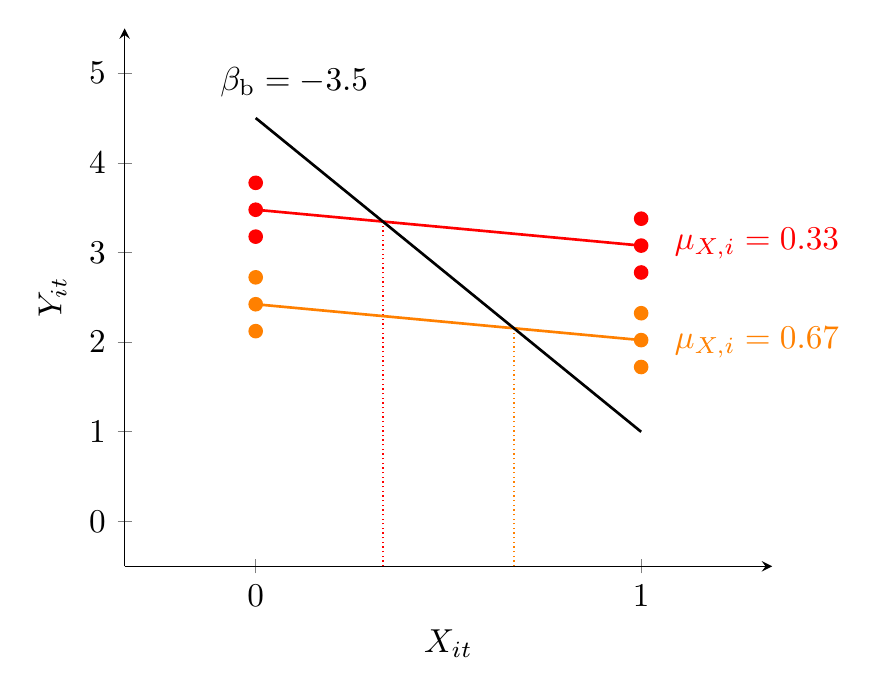
\begin{tikzpicture}[scale=1.2]
    \begin{axis}[
        axis x line=left, 
        axis y line=left, 
        xlabel={$X_{it}$}, ylabel={$Y_{it}$},
        xmin=-0.2, xmax=1.2, ymin=0, ymax=5,
        xtick={0,1},
        ytick={0,1,2,3,4,5},
        enlargelimits=true,
        clip=false,
        xshift=-15mm
    ]

    \pgfmathsetmacro{\gammaZero}{4.5}
    \pgfmathsetmacro{\gammaOne}{-3.1}
    \pgfmathsetmacro{\betaOne}{-0.4}
    \pgfmathsetmacro{\betaB}{-3.5}

    % === Person with mu_X = 0.33 ===
    \pgfmathsetmacro{\muXone}{0.33}
    \pgfmathsetmacro{\intOne}{\gammaZero + \gammaOne*\muXone}
    \addplot[thick, red] coordinates {
        (0, {\intOne + \betaOne*0})
        (1, {\intOne + \betaOne*1})
    };
    \addplot[only marks, red] coordinates {
        (0, {\intOne + \betaOne*0})
        (0, {\intOne + \betaOne*0.75})
        (0, {\intOne + \betaOne*-0.75})
        (1, {\intOne + \betaOne*0.25})
        (1, {\intOne + \betaOne*1})
        (1, {\intOne + \betaOne*1.75})
    };
    \addplot[densely dotted, thin, red] coordinates {
        (\muXone, -0.5)
        (\muXone, {\gammaZero + \betaB*\muXone})
    };

    % === Person with mu_X = 0.67 ===
    \pgfmathsetmacro{\muXtwo}{0.67}
    \pgfmathsetmacro{\intTwo}{\gammaZero + \gammaOne*\muXtwo}
    \addplot[thick, orange] coordinates {
        (0, {\intTwo + \betaOne*0})
        (1, {\intTwo + \betaOne*1})
    };
    \addplot[only marks, orange] coordinates {
        (0, {\intTwo + \betaOne*0})
        (0, {\intTwo + \betaOne*0.75})
        (0, {\intTwo + \betaOne*-0.75})
        (1, {\intTwo + \betaOne*0.25})
        (1, {\intTwo + \betaOne*1})
        (1, {\intTwo + \betaOne*1.75})
    };
    \addplot[densely dotted, thin, orange] coordinates {
        (\muXtwo, -0.5)
        (\muXtwo, {\gammaZero + \betaB*\muXtwo})
    };

    % === Between-person regression line ===
    \addplot[thick, black, domain=0:1] {\gammaZero + \betaB*x};

    % === Labels ===
    \node[red] at (axis cs:1.3,3.1) {$\mu_{X,i}=0.33$};
    \node[orange] at (axis cs:1.3,2.0) {$\mu_{X,i}=0.67$};
    \node[black] at (axis cs:0.1,4.9) {$\beta_\text{b} = -3.5$};

    \end{axis}
\end{tikzpicture}

    \label{fig:withinbetween-binxconty}
    \begin{figurenote}
        The solid black slope represents the between-person effect and the colored slopes the within-cluster effects. The X-axis simultaneously represents $X_{it}$ for the within-slope and $\mu_{X,i}$ for the between-slope; and the Y-axis represents $Y_{it}$ for the within slope and $Y_i$ for the between-slope. Dots reflect possible datapoints and diamonds reflect the position of $\mu_{X,i}$ on the within-person slope.
    \end{figurenote}
\end{center}

\subsection{Multilevel Logistic Model}

Dichotomous outcomes necessitate the use of non-linear models, as they represent probabilities rather than continuous values. Because probability is inherently bounded between 0 and 1, a linear function is unsuitable for prediction. Instead, we employ a logistic transformation, mapping probabilities onto the unbounded log-odds scale via the logit function:
\begin{equation}
    \text{logit}(p) = \log\left(\frac{p}{1 - p}\right)
\end{equation}
As a consequence, the parameters and partition of variance do not have the intuitive interpretation of the MLM \parencite{merlo_brief_2006}.The fixed effects now correspond to changes in the log-odds of the outcome, rather than direct changes in the outcome itself, as in a linear model. To facilitate interpretation, we can convert log-odds back into probabilities using the inverse logit transformation:
\[
p = \frac{e^{\text{logit}(p)}}{1 + e^{\text{logit}(p)}}
\]
Using this formula, we can establish that a log-odds of 0 corresponds to a 50\% probability, positive log-odds indicate a probability greater than 50\% and negative log-odds indicate a probability less than 50\%.

\subsection{DGM 3: Continuous Predictor and Dichotomous Outcome}

Compared to an MLM with a continuous predictor and outcome, introducing a dichotomous outcome modifies only the within-person equation, while the between-person equation remains structurally identical (see Figures~\ref{fig:contxy} and~\ref{fig:contxdichy}). Consider a scenario where we examine the relationship between time spent in bed (\(X_{it}\)) and the probability of experiencing interpersonal conflict (\(Y_{it}\)), coded as 1 if conflict is reported and 0 otherwise. The model is expressed as:
\begin{align}
\label{eqn:logityit-cont}
\text{logit}(P(Y_{it} = 1)) &= \beta_{0i} + \beta_1 X_{it}, \\
\label{eqn:beta0-cont}
\beta_{0i} &= \gamma_{00} + \gamma_{01} \mu_{X,i} + u_{0i}.
\end{align}
By substituting the between-person equation into the within-person equation, we obtain the combined model:
\begin{equation}
\text{logit}(P(Y_{it} = 1)) = \gamma_{00} + \gamma_{01} \mu_{X,i} + u_{0i} + \beta_1 X_{it}.
\end{equation}

% The predictor \( X_{it} \) is generated identically to the multilevel linear model with continuous predictor (see equations~\ref{eqn:xbetweencontxy},~\ref{eqn:xwithincontxy}). Thus, the fixed effects have the same interpretation as in the MLM, but now represent effects on the log-odds scale. The intercept \( \gamma_{00} \) represents the expected log-odds of experiencing interpersonal conflict for an individual whose cluster mean $\mu_{X,i}$ is zero, while \( \beta_1 \) quantifies how deviations from a person’s usual sleep duration (\(X_{w,it} = X_{it} - \mu_{X,i}\)) relate to changes in the log-odds of interpersonal conflict. The coefficient \( \gamma_{01} \) captures the degree to which the between-person effect---the association between a person’s typical sleep duration (\( \mu_{X,i} \)) and log-odds of interpersonal conflict---differs from the within-person effect. The between-person effect $\beta_\text{b} = \gamma_{01} + \beta_\text{w}$ describes whether individuals who have a high average sleep duration are overall more frequently involved in interpersonal conflict.

% It tends to be more insightful, however, to convert the log-odds to probabilities. To illustrate, Suppose the true data-generating process assumes $\gamma_{00} = -2$, \(\beta_\text{w} = -0.4\) and \(\gamma_{01} = 0.6\) and \(\beta_\text{b} = 0.6 + 0.4 = 1\). Then we have:
% \begin{equation}
% \text{logit}(P(Y_{it} = 1)) = -2 + 0.6 \mu_{X,i} - 0.4 X_{it} + u_{0i}.
% \end{equation}
% Since \(\beta_\text{w} < 0\) , we know that an increase in sleep duration for a given person tends to result in fewer conflicts; whereas \(\beta_\text{b} > 0\) implies that people who sleep more overall tend to be more frequently involved in conflict. Let us consider an example for the within-person effect. Consider that James has an average sleep duration of \(\mu_{X,i} = 6\) hours and sleeps 6 hours on a particular night such that \(X_{w,it} = 6 - 6 = 0\). Suppose his baseline log-odds of conflict (when \(X_{it} = \mu_{X,i}\)) is:
% \begin{equation}
% \text{logit}(P(Y_{it} = 1)) = -2 + 0.6 \cdot 6 - 0.4 \cdot 0  + u_{0i}.
% \end{equation}
% Due to the non-linear function, to proceed we must now assume that we are dealing with an individual with the average individual, who has $u_{0i} = 0$:
% \begin{equation}
% \text{logit}(P(Y_{it} = 1)) = -2 + 3.6  = 1.6
% \end{equation}
% To convert this to probability, we apply the inverse logit transformation:
% \[
% P(Y_{it} = 1) = \frac{e^{1.6}}{1 + e^{1.6}} \approx \frac{4.95}{1 + 4.95} \approx 0.83.
% \]
% Now, if James sleeps one hour longer than usual (\(X_{it} = \mu_{X,i} + 1 = 7\)), his predicted log-odds change by \(\beta_\text{w} = -0.4\):
% \[
% \text{logit}(P(Y_{it} = 1)) = 1.6 - 0.4 \cdot 1 = 1.2.
% \]
% Converting this back to probability:
% \[
% P(Y_{it} = 1) = \frac{e^{1.2}}{1 + e^{1.2}} \approx \frac{3.32}{1 + 3.32} \approx 0.77.
% \]
% Thus, increasing sleep by one hour reduces the probability of experiencing conflict from 83\% to 77\%, demonstrating the within-person effect.

% Now, let’s examine the between-person effect by considering two individuals who differ in their average sleep: James sleeps 6 hours on average (\(\mu_{X,i} = 6\)) and Bruno sleeps 8 hours on average (\(\mu_{X,i} = 8\)). We have already seen that James, who sleeps 6 hours has a probability of experiencing conflict of 83\%. Now consider that Bruno sleeps 8 hours on a particular night and that there is no unobserved variability ($u_{0i} = 0$), so that his logg-odds of conflict are:
% \[
% \text{logit}(P(Y_{it} = 1)) = \gamma_{00} + 0.6(8) = -2 + 4.8 = 2.8.
% \]
% Converting to probability:
% \[
% P(Y_{it} = 1) = \frac{e^{2.8}}{1 + e^{2.8}} \approx \frac{16.45}{1 + 16.45} \approx 0.94.
% \]
% So, Bruno who sleeps 8 hours has a 94\% probability of experiencing interpersonal conflict, compared to James who sleeps 6 hours, whose probability is 83\%. This reflects the between-person effect: individuals who generally spend more time in bed tend to have a higher overall probability of conflict. 

\begin{center}
    \captionof{figure}{Within- and Between-Person Effects of Continuous Predictor and Binary Outcome}

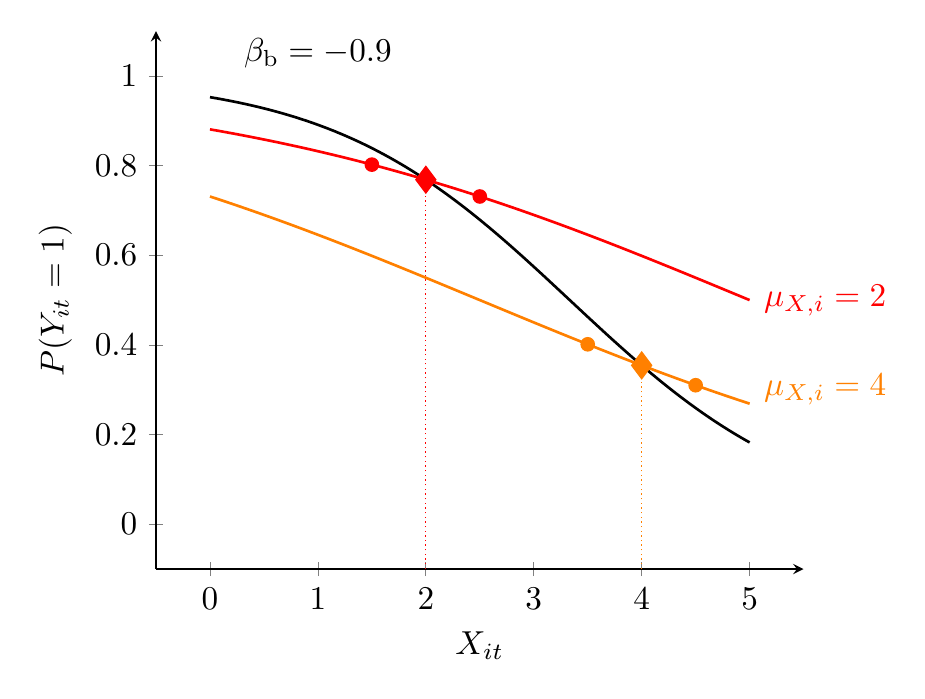
\begin{tikzpicture}[scale=1.2]
    \begin{axis}[
        axis x line=left, axis y line=left,
        xlabel={$X_{it}$}, ylabel={$P(Y_{it} = 1)$},
        xmin=0, xmax=5, ymin=0, ymax=1,
        % legend pos=south west,
        samples=200,
        domain=0:5,
        ytick={0,0.2,0.4,0.6,0.8,1},
        xtick={0,1,2,3,4,5},
        clip=false,
        enlargelimits=true
    ]
    
    % Parameters
    \pgfmathsetmacro{\gammaZero}{3}
    \pgfmathsetmacro{\gammaOne}{-0.5}
    \pgfmathsetmacro{\betaOne}{-0.4}
    \pgfmathsetmacro{\betaB}{-0.9}
    
    % Person 1: mu_X = 2
    \pgfmathsetmacro{\muXone}{2}
    \pgfmathsetmacro{\intOne}{\gammaZero + \gammaOne*\muXone}
    \addplot[red, thick] {1 / (1 + exp(-(\intOne + \betaOne*x)))};
    \addplot[only marks, mark=*, red] coordinates {
        (1.5, {1 / (1 + exp(-(\intOne + \betaOne*1.5)))})
        (2.5, {1 / (1 + exp(-(\intOne + \betaOne*2.5)))})
    };
    \addplot[only marks, mark=diamond*, mark size=4pt, red] coordinates {
        (2, {1 / (1 + exp(-(\intOne + \betaOne*2)))})
    };
    \addplot[densely dotted, thin, red] coordinates {
        (\muXone, -0.1)
        (\muXone, {1 / (1 + exp(-(\intOne + \betaOne*\muXone)))})
    };
    
    
    % Person 2: mu_X = 4
    \pgfmathsetmacro{\muXtwo}{4}
    \pgfmathsetmacro{\intTwo}{\gammaZero + \gammaOne*\muXtwo}
    \addplot[orange, thick] {1 / (1 + exp(-(\intTwo + \betaOne*x)))};
    \addplot[only marks, mark=*, orange] coordinates {
        (3.5, {1 / (1 + exp(-(\intTwo + \betaOne*3.5)))})
        (4.5, {1 / (1 + exp(-(\intTwo + \betaOne*4.5)))})
    };
    \addplot[only marks, mark=diamond*, mark size=4pt, orange] coordinates {
        (4, {1 / (1 + exp(-(\intTwo + \betaOne*4)))})
    };
    \addplot[densely dotted, thin, orange] coordinates {
    (\muXtwo, -0.1)
    (\muXtwo, {1 / (1 + exp(-(\intTwo + \betaOne*\muXtwo)))})
    };
    
    % Between-person curve
    \addplot[black, thick] {1 / (1 + exp(-(\gammaZero + \betaB*x)))};

    % === Labels ===
    \node[red] at (axis cs:5.7,0.5) {$\mu_{X,i}=2$};
    \node[orange] at (axis cs:5.7,0.3) {$\mu_{X,i}=4$};
    \node[black] at (axis cs:1,1.05) {$\beta_\text{b} = -0.9$};
    
    
    \end{axis}
\end{tikzpicture}

    \label{fig:withinbetween-contxbiny}
    \begin{figurenote}
        The solid black slope represents the between-person effect and the colored slopes the within-cluster effects. The X-axis simultaneously represents $X_{it}$ for the within-slope and $\mu_{X,i}$ for the between-slope; and the Y-axis represents $Y_{it}$ for the within slope and $Y_i$ for the between-slope. Dots reflect possible datapoints and diamonds reflect the position of $\mu_{X,i}$ on the within-person slope.
    \end{figurenote}
\end{center}

\subsection{DGM 4: Dichotomous Predictor and Outcome}

When replacing the predictor in the multilevel logistic model with a dichotomous one, the within-person equation remains the same (see equation~\ref{eqn:logityit-cont}), but the between-person model changes (compare Figures~\ref{fig:contxdichy} and~\ref{fig:dichxy}):
\begin{align}
\label{eqn:beta0-dich}
\beta_{0i} &= \gamma_{00} + \gamma_{01} \pi_{Xi} + u_{0i},
\end{align}
where \( \pi_{Xi} \) represents the probability of \( X_{it} = 1 \) for individual \( i \). The composite model becomes:
\begin{equation}
\text{logit}(P(Y_{it} = 1)) = \gamma_{00} + \gamma_{01} \pi_{Xi} + u_{0i} + \beta_1 X_{it}.
\end{equation}
where the predictor \( X_{it} \) is generated identically to the MLM with a dichotomous predictor (see equations~\ref{eqn:binxconty-Xgeneration1},~\ref{eqn:binxconty-Xgeneration2} and~\ref{eqn:binxconty-Xgeneration3}).  Thus, the fixed effects have the same interpretation as in the MLM, but now represent effects on the log-odds scale.

 % The intercept \( \gamma_{00} \) represents the expected log-odds of interpersonal conflict for an individual who never engages in mindfulness ($\pi_{Xi} = 0$) . The within-person effect \( \beta_1 \) quantifies how an individual's likelihood of experiencing conflict changes on days when they engage in mindfulness practice versus days when they do not. The contextual effect \( \gamma_{01} \) captures the degree to which the between-person effect---the association between a person's long-term tendency to engage in mindfulness \( \pi_{Xi} \) and their overall tendency to experience conflict---differs from the within-person effect. The between-person effect $\beta_\text{b} = \gamma_{01} + \beta_\text{w}$ describes whether individuals who generally engage in mindfulness more frequently experience a systematically different likelihood of being involved in conflict compared to those who rarely or never engage in the practice.  

 It tends to be more insightful, however, to convert the log-odds to probabilities. To illustrate, Suppose the true data-generating process assumes $\gamma_{00} = -2$, \(\beta_\text{w} = -0.4\) and \(\gamma_{01} = 0.6\) and \(\beta_\text{b} = 0.6 + 0.4 = 1\). As can be observed in Figure~\ref{fig:withinbetween-binxy}, when coefficient values are similar to the continuous case, we obtain slopes that more closely resemble a linear relationship rather than a pronounced S-curve (see Figure~\ref{fig:withinbetween-contxbiny}). This is because the variation in $X_{it}$ is much lower. Since \(\beta_\text{w} < 0\), this suggests that individuals tend to have a smaller probability of experiencing interpersonal conflict on days they engage in mindfulness; whereas \(\beta_\text{b} > 0\) implies that those who engage in mindfulness more frequently tend to have a higher overall probability of conflict.

 \begin{center}
    \captionof{figure}{Within- and Between-Person Effects of Binary Predictor and Outcome}

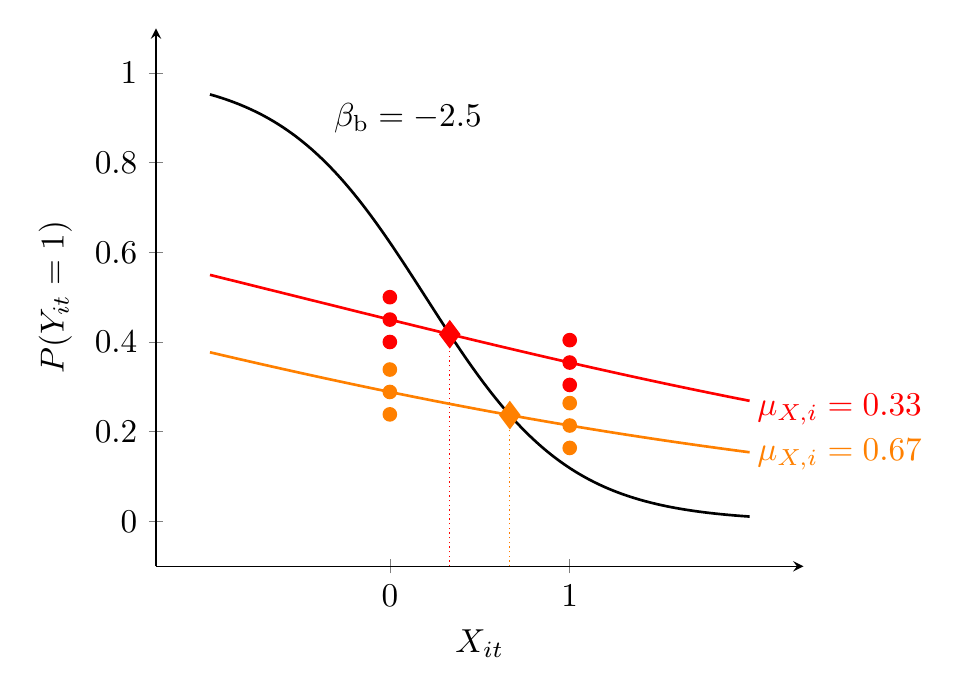
\begin{tikzpicture}[scale=1.2]
    \begin{axis}[
        axis x line=left, axis y line=left,
        xlabel={$X_{it}$}, ylabel={$P(Y_{it} = 1)$},
        xmin=-1, xmax=2, ymin=0, ymax=1,
        % legend pos=south west,
        samples=200,
        domain=-1:2,
        ytick={0,0.2,0.4,0.6,0.8,1},
        xtick={0,1},
        clip=false,
        enlargelimits=true
    ]
    
    % Parameters
    \pgfmathsetmacro{\gammaZero}{0.5}
    \pgfmathsetmacro{\gammaOne}{-2.1}
    \pgfmathsetmacro{\betaOne}{-0.4}
    \pgfmathsetmacro{\betaB}{-2.5}
    
    % Person 1: mu_X = 0.333
    \pgfmathsetmacro{\muXone}{0.333}
    \pgfmathsetmacro{\intOne}{\gammaZero + \gammaOne*\muXone}
    \addplot[red, thick] {1 / (1 + exp(-(\intOne + \betaOne*x)))};
    \addplot[only marks, mark=diamond*, mark size=4pt, red] coordinates {
        (0.333, {1 / (1 + exp(-(\intOne + \betaOne*0.333)))})
    };
    \addplot[only marks, mark=*, red] coordinates {
        (0, {1 / (1 + exp(-(\intOne + \betaOne*0)))})
        (0, {1 / (1 + exp(-(\intOne + \betaOne*0))) + 0.05})
        (0, {1 / (1 + exp(-(\intOne + \betaOne*0))) - 0.05})
        (1, {1 / (1 + exp(-(\intOne + \betaOne*1)))})
        (1, {1 / (1 + exp(-(\intOne + \betaOne*1))) + 0.05})
        (1, {1 / (1 + exp(-(\intOne + \betaOne*1))) - 0.05})
    };
    \addplot[densely dotted, thin, red] coordinates {
        (\muXone, -0.1)
        (\muXone, {1 / (1 + exp(-(\intOne + \betaOne*\muXone)))})
    };
    
    % Person 2: mu_X = 0.667
    \pgfmathsetmacro{\muXtwo}{0.667}
    \pgfmathsetmacro{\intTwo}{\gammaZero + \gammaOne*\muXtwo}
    \addplot[orange, thick] {1 / (1 + exp(-(\intTwo + \betaOne*x)))};
    \addplot[only marks, mark=diamond*, mark size=4pt, orange] coordinates {
        (0.667, {1 / (1 + exp(-(\intTwo + \betaOne*0.667)))})
    };
    \addplot[only marks, mark=*, orange] coordinates {
        (0, {1 / (1 + exp(-(\intTwo + \betaOne*0)))})
        (0, {1 / (1 + exp(-(\intTwo + \betaOne*0))) + 0.05})
        (0, {1 / (1 + exp(-(\intTwo + \betaOne*0))) - 0.05})
        (1, {1 / (1 + exp(-(\intTwo + \betaOne*1)))})
        (1, {1 / (1 + exp(-(\intTwo + \betaOne*1))) + 0.05})
        (1, {1 / (1 + exp(-(\intTwo + \betaOne*1))) - 0.05})
    };
    
    \addplot[densely dotted, thin, orange] coordinates {
    (\muXtwo, -0.1)
    (\muXtwo, {1 / (1 + exp(-(\intTwo + \betaOne*\muXtwo)))})
    };
    
    % Between-person curve
    \addplot[black, thick] {1 / (1 + exp(-(\gammaZero + \betaB*x)))};

    % === Labels ===
    \node[red] at (axis cs:2.5,0.25){$\mu_{X,i}=0.33$};
    \node[orange] at (axis cs:2.5,0.15) {$\mu_{X,i}=0.67$};
    \node[black] at (axis cs:0.1,0.9) {$\beta_\text{b} = -2.5$};
    
    \end{axis}
\end{tikzpicture}

    \label{fig:withinbetween-binxy}
    \begin{figurenote}
        The solid black slope represents the between-person effect and the colored slopes the within-cluster effects. The X-axis simultaneously represents $X_{it}$ for the within-slope and $\mu_{X,i}$ for the between-slope; and the Y-axis represents $Y_{it}$ for the within slope and $Y_i$ for the between-slope. Dots reflect possible datapoints and diamonds reflect the position of $\mu_{X,i}$ on the within-person slope.
    \end{figurenote}
\end{center}

\section{Modeling Methods}

\ldots

\begin{itemize}
    \item Within the multilevel modeling literature, the importance of separating the within-cluster from the between-cluster slope for \textit{continuous predictors} has been repeatedly stressed by many \parencite[e.g.,][]{enders_centering_2007, kreft_effect_1995, raudenbush_hierarchical_2002}, to the extent that it has now become a general consensus among social researchers. The primary reason for this is that failing to account for contextual effects—where the relationship between a predictor and an outcome differs across levels—leads to an uninterpretable blend of within- and between-person slopes \parencite[139]{raudenbush_hierarchical_2002}.  The main concern here is that it is the within effect which is commonly of interest and relevant for causal interpretation.
    \item Models were parametrized as Mundlak's contextual model \parencite[]{mundlak_pooling_1978}, implying they include an uncentered predictor and cluster mean as predictors.
    \item To better understand why we obtain biased parameter estimates when failing to account for the contextual effect, we should examine the path diagram (see Figure~\ref{fig:contxy}). This clarifies how \( \mu_X \) functions as a confounder (i.e., shared cause) in the relationship between \( X_{it} \) and $Y_{it}$ (through \( \beta_{0i} \)). Notably, if there is no contextual effect (i.e., \( \gamma_{10} = 0 \)), the pathway from \( \mu_X \) to the random intercept vanishes, eliminating this confounding. Similarly, if there is no between-person variation in \( \mu_X \), all outgoing paths from \( \mu_X \) disappear, again removing the confounding effect. However, when there is between-person variation and a contextual effect, it is essential to control for \( \mu_X \) in some form to ensure accurate inference.
    \item "between-subjects and within-subjects relationships can have very different magnitudes and even different signs, and can result in aconceptual error that is sometimes called an ecological fallacy, wherein relationships at the upper level of analysis are confused with those at the lower level (Robinson, 1950)." \parencite[p. 71]{bolger_intensive_2013}
\end{itemize}


\subsection{Multilevel Linear and Logistic Models}

If within- and between-person slopes are identical or only one of them exists, this issue is negligible. However, in most research, we cannot a priori exclude the possibility of a contextual effect. Conversely, contextual effects are often the very reason for using MLMs, making their explicit separation crucial. Let us consider the case of a simple MLM with a random intercept and raw level 1 predictor $X_{it}$, where the model is formulated as:
\begin{align}
Y_{it} &= \beta_{0i} + \beta_1 X_{it} + e_{it},  \\
\beta_{0i} &= \gamma_{00} + u_{0i}.
\end{align}
Substituting the between-person equation into the within-person equation gives:
\begin{equation}
Y_{it} = \gamma_{00} + u_{0i} + \beta_ 1 X_{it} + e_{it}.
\end{equation}
In this case, the resulting estimate of $\beta_1$ is a weighted sum of the within- and between-person slopes, where the weight depends on the number of timepoints $T$ \parencite{mundlak_pooling_1978}. The estimate is more heavily influenced by the within-person effect with a greater number of timepoints. To correctly estimate both effects, several approaches have been developed.

\subsubsection{Multilevel Linear Model}

\paragraph{Within-Person Centered Predictor}

One solution is centering the predictor $X$ within clusters, yielding the cluster mean $\bar{X_i}$ and the within-person centered predictor $(X_{it} - \bar{X_i})$. This method ensures that the within-person slope is not confounded\footnote{We can see this in Figure \ref{fig:contxy}, where $\mu_X$ is a confounder in the relationship between each observation of $X_{it}$ and the random intercept $\beta_{0i}$.} by between-person differences \parencite[e.g.,][]{hoffman_longitudinal_2015, kreft_effect_1995, raudenbush_hierarchical_2002}. The model is then specified as:
\begin{align}
Y_{it} &= \beta_{0i} + \beta_\text{w} (X_{it}- \bar{X_i}) + e_{it},  \\
\beta_{0i} &= \gamma_{00} + u_{0i}.
\end{align}
Substituting the second equation into the first gives:
\begin{equation}
Y_{it} = \gamma_{00} + u_{0i} + \beta_\text{w} (X_{it}- \bar{X_i}) + e_{it}.
\end{equation}
Since $(X_{it} - \bar{X_i})$ contains no between-person variance, $\beta_\text{w}$ estimates the within-person slope. To obtain the between-person slope $\beta_\text{b}$, the cluster mean $\bar{X_i}$ is added as a predictor:
\begin{align}
\beta_{0i} &= \gamma_{00} + \beta_\text{b} \bar{X_i} + u_{0i}.
\end{align}
The full model then becomes:
\begin{equation}
Y_{it} = \gamma_{00} + \beta_\text{b} \bar{X_i} + u_{0i} + \beta_\text{w} (X_{it} - \bar{X_i}) + e_{it}.
\end{equation}
\paragraph{Mundlak's Contextual Model}

An alternative approach, known as the Mundlak model \parencite{mundlak_pooling_1978}, retains the raw predictor $X_{it}$ in the within-person equation while including $\bar{X_i}$ in the between-person equation:
\begin{align}
Y_{it} &= \beta_{0i} + \beta_\text{w} X_{it} + e_{it}, \\
\beta_{0i} &= \gamma_{00} + \gamma_{01} \bar{X_i} + u_{0i}.
\end{align}
Substituting the second equation into the first gives:
\begin{equation}
Y_{it} = \gamma_{00} + \gamma_{01} \bar{X_i} + u_{0i} + \beta_\text{w} X_{it} + e_{it}.
\end{equation}
Because $\bar{X_i}$ and $X_{it}$ are correlated, their coefficients reflect only their unique contributions. Thus, $\beta_\text{w}$ estimates the within-person slope, while $\gamma_{01}$ represents the difference between the within- and between-person slopes ($\beta_\text{b} - \beta_\text{w}$), also known as the contextual effect \parencite{hoffman_longitudinal_2015, raudenbush_hierarchical_2002}.

\paragraph{Latent Mean Centering and Lüdtke's Bias}

Until now, the discussed two multilevel approaches utilized $\bar{X_i}$---the sample mean per person across timepoints on the predictor $X_{it}$. In the presence of contextual effects, \textcite{ludtke_multilevel_2008}  shows that the observed mean centering method yields biased results, especially concerning the between-person slope. As shown by \parencite[]{asparouhov_latent_2019}, the bias in $\beta_\text{b}$ tends to increase with a greater contextual effect, smaller between-person variance in the predictor and smaller number of timepoints $T$. This bias can be avoided by employing latent mean centering, where we assume a distribution underlying the cluster means. While this method is more robust to bias, it is not part of many software implementations of the multilevel linear model (e.g., the \texttt{lme4} package in R).

% \begin{equation}
%     \frac{(\beta_\text{w}-\beta_\text{b}) \psi_W / T}{\psi_B + \psi_W / T}
% \end{equation}
% where $\psi_W$ is the within-person variance of $X$, $\psi_B$ is the between-person variance of $X$ and $T$ is the total number of timepoints. 

\paragraph{Centering Dichotomous Predictors}

When predictors are dichotomous, the interpretation of within- and between-person slopes changes: rather than representing continuous variation, a dichotomous predictor indicates the presence or absence of a characteristic. This requires a different conceptualization of within-person change and between-person differences.

If the predictor \( X_{it} \) is dichotomous (e.g., an indicator for whether an event occurred), within-person centering still involves computing the cluster mean \( \bar{X_i} \), but its meaning differs. Since \( \bar{X_i} \) now refers to the proportion of event occurrence across timepoints, the term \( (X_{it} - \bar{X_i}) \) reflects deviations from an individual's proportion of having of experienced the event rather than fluctuations around a continuous mean. Consequently, the within-person slope \( \beta_\text{w} \) represents how changes in the predictor status (e.g., experiencing the event vs. not experiencing it) are associated with changes in the outcome within individuals. The between-person slope \( \beta_\text{b} \) then reflects how differences in average event occurrence across observed timepoints relate to differences in the outcome between individuals. 

Just as in the continuous case, the contextual effect \( \gamma_{01} \) now represents the extent to which the between-person association deviates from the within-person effect.

\begin{itemize}
    \item explain that in the case of a dichotomous predictor, the contextual effect is often of greater interest than the between-person effect
\end{itemize}

Another practical consideration is that in models with a dichotomous predictor, interpretation can be affected by the distribution of \( X_{it} \). If the event is rare, within-person variation may be limited, leading to unstable estimates of \( \beta_\text{w} \). Additionally, if individuals are measured on few timepoints, the number of possible proportions that they can have will be limited to $T+1$. For instance, if we measure individuals on 5 timepoints, the only possible values for \( \bar{X_i} \) are $0, 0.2, 0.4, 0.6, 0.8, 1$.

\subsubsection{Multilevel Logistic Model}

The multilevel linear model falls under the umbrella of the generalized linear model, where several other families of distributions (e.g., binomial) and link functions are available. In this general framework, the MLM is a GLMM with a gaussian (i.e., normal) distribution and identity link. When modeling dichotomous outcomes (e.g., relationship conflict), the binomial family is used, often with a logit link  on the response variable. 

\begin{enumerate}
    \item Explain what changes when we are modeling a dichotomous as opposed to a continuous outcome. More specifically, how the within and between thinking relates to multilevel models with dichotomous outcomes, how this changes the interpretation and if this introduces challenges.
    \item with a dichotomous outcome the random intercept variance $\sigma^2_{u0}$ represents variation in log-odds across clusters rather as opposed to a continuous outcome, where it represents variation in the outcome directly.
\end{enumerate}

\paragraph{Within-Person Centered Predictor}

In the context of binary outcomes, the multilevel logistic model can be extended to disentangle within- and between-person effects using within-person centering. The probability of a binary outcome \( Y_{it} \in \{0,1\} \) is modeled via the logit link:
\begin{equation}
\text{logit}(\Pr(Y_{it} = 1)) = \gamma_{00} + u_{0i} + \beta_\text{w} (X_{it} - \bar{X_i}).
\end{equation}
Here, \( \beta_\text{w} \) captures the within-person effect of \( X \) on the log-odds of the outcome, unconfounded by between-person variation. To recover the between-person effect, the person-level mean \( \bar{X_i} \) is added as a level-2 predictor:
\begin{equation}
\text{logit}(\Pr(Y_{it} = 1)) = \gamma_{00} + \beta_\text{b} \bar{X_i} + u_{0i} + \beta_\text{w} (X_{it} - \bar{X_i}).
\end{equation}
This decomposition facilitates distinct estimation of within- and between-person contributions on the log-odds scale.

\paragraph{Mundlak’s Contextual Model}

Alternatively, the Mundlak model retains the raw time-varying predictor \( X_{it} \) and introduces the person-mean \( \bar{X_i} \) as a contextual effect:
\begin{equation}
\text{logit}(\Pr(Y_{it} = 1)) = \gamma_{00} + \gamma_{01} \bar{X_i} + u_{0i} + \beta_\text{w} X_{it}.
\end{equation}
As in the linear case, this model yields an implied between-person effect of \( \beta_\text{b} = \gamma_{01} + \beta_\text{w} \). While interpretation on the log-odds scale complicates direct comparisons, this approach preserves interpretability and enables inclusion of contextual effects without altering the level-1 predictor.


\subsection{Generalized Estimating Equations}

\subsubsection{Conceptual Overview}

% \begin{enumerate}
%     \item Explain the general formulation and idea behind the GEE approach
%     \item Introduce different common working correlation structures and robustness against misspecification
%     \item Add 1 or 2 sentences on the marginal/conditional effect conceptualization that is more common in other fields.
%     \item You cannot be completely sure the model converged, which is a potential issue.
% \end{enumerate}

The Generalized Estimating Equations (GEE) approach, introduced by \textcite{liang_longitudinal_1986}, is a semi-parametric method for analyzing correlated data, such as repeated measures or clustered observations. Unlike, the multilevel model, GEEs do not entail random effects. As random effects impose extra assumptions, this means that modeling with GEE requires fewer assumptions compared to multilevel models \parencite[]{mcneish_measurement_2021}.

The general formulation of a GEE follows from the standard generalized linear model (GLM) framework:
\begin{equation}
E(Y_{it} | X_{it}) = g^{-1}(X_{it}^T \beta),
\end{equation}
where \( g(\cdot) \) is the canonical link function corresponding to the chosen distribution (e.g., identity for Gaussian, logit for binomial), \( X_{it} \) is a vector of covariates, and \( \beta \) is the vector of regression coefficients. Rather than specifying a full likelihood function as in the multilevel model, GEE estimates parameters by solving the quasi-likelihood estimating equation:
\begin{equation}
\sum_{i=1}^{N} D_i^T V_i^{-1} (Y_i - \mu_i) = 0,
\end{equation}
where \( D_i = \frac{\partial \mu_i}{\partial \beta} \) is the derivative of the mean function, and \( V_i \) is the working covariance matrix of the repeated measures. The estimation procedure in GEE follows an iterative process:
\begin{enumerate}
    \item Specify the Mean Structure: Define the expected response \( E(Y_{it} | X_{it}) \) using an appropriate link function based on the assumed distribution of the outcome variable.
    \item Specify the Working Correlation Structure: Choose a working correlation matrix \( R(\alpha) \) to model the within-cluster dependence. Common choices include independent, exchangeable, autoregressive (AR1), and unstructured correlations.
    \item Initial Estimation: Treating the data as if they were independent, estimate the regression coefficients \( \beta \) using standard GLM techniques.
    \item Estimate the Parameters in $K$: Compute initial estimates of the correlation parameters using the estimated residual errors from the GLM.
    \item Estimate the Variance Components: Compute the working covariance matrix \( V_i \) using the current estimate of \( \beta \) and the assumed correlation structure.
    \item Update the Regression Coefficients: Solve the quasi-likelihood estimating equation iteratively to refine \( \beta \), incorporating the updated covariance matrix.
    \item After convergence is reached, compute the cluster-robust standard errors. If convergence issues arise, consider alternative correlation structures or estimation methods.
\end{enumerate}

Convergence is proclaimed when either the change in parameter estimations is less than a specified criterion or the change in the sum of squared deviances is less than a provided criterion. \parencite[p. 92]{hardin_generalized_2012}. 

As extra step, GEE requires us to specify a working correlation matrix for the association among observations from each subject \parencite[]{diggle_analysis_2002}. However, GEE is robust against most misspecifications \parencite[]{zeger_models_1988, ballinger_using_2004}. Common choices include (1) exchangeable, (2) independence and (3) autoregressive lag (1) (AR(1)). The exchangeable structure assumes a constant correlation $\alpha$ among all observations $Y_{it}$ within the same cluster $i$:
\[
R = 
\begin{bmatrix}
1 & \alpha & \alpha & \alpha & \alpha \\
\alpha & 1 & \alpha & \alpha & \alpha \\
\alpha & \alpha & 1 & \alpha & \alpha \\
\alpha & \alpha & \alpha & 1 & \alpha \\
\alpha & \alpha & \alpha & \alpha & 1
\end{bmatrix}
\]
The independence structure assumes no correlation between observations $Y_{it}$ within the same cluster:
\[
R = 
\begin{bmatrix}
1 & 0 & 0 & 0 & 0 \\
0 & 1 & 0 & 0 & 0 \\
0 & 0 & 1 & 0 & 0 \\
0 & 0 & 0 & 1 & 0 \\
0 & 0 & 0 & 0 & 1
\end{bmatrix}
\]
The AR(1) structure assumes correlations decay exponentially as a function of time as \( \alpha^{|t-t'|} \):
\[
R = 
\begin{bmatrix}
1 & \alpha & \alpha^2 & \alpha^3 & \alpha^4 \\
\alpha & 1 & \alpha & \alpha^2 & \alpha^3 \\
\alpha^2 & \alpha & 1 & \alpha & \alpha^2 \\
\alpha^3 & \alpha^2 & \alpha & 1 & \alpha \\
\alpha^4 & \alpha^3 & \alpha^2 & \alpha & 1
\end{bmatrix}
\]
Generalized estimating equations are often referred to as \textit{marginal} models, as they yield the marginal expectation of an outcome $Y$ as a function of explanatory variables \parencite[]{diggle_analysis_2002}. This is directly opposed by methods---such as the multilevel model---that model random effects, which yield the conditional-on-the-random-effect expectation. This means that the coefficients in a GEE analysis describe the average relationship between predictors and outcomes across the population, rather than for the average individual. This distinction is particularly relevant in fields such as epidemiology and biostatistics, where marginal interpretations are often preferred.

A key limitation of generalized estimating equations (GEE) is the absence of a fully specified likelihood function. This precludes the use of likelihood-based model fit indices such as AIC, BIC, or likelihood ratio tests, which require a properly defined likelihood. Furthermore, because GEE does not optimize a likelihood function, standard convergence diagnostics are less informative. Estimation typically relies on iterative reweighted least squares (IRLS), but this algorithm does not guarantee convergence to a global optimum, nor does it necessarily indicate whether a stable solution has been reached. These limitations are especially pronounced in small samples or when data exhibit high within-cluster correlation, where non-convergence may yield infinite or unstable estimates. Researchers are advised to closely monitor convergence diagnostics and, in cases of instability, to (a) explore alternative working correlation structures or (b) consider alternative estimators for the dispersion parameter \parencite[p. 97]{hardin_generalized_2012}.

\subsubsection{Centering Approaches}

\paragraph{Identity Link}

When the identity link is used with GEE, the marginal expectation of the outcome \( Y_{it} \) is modeled as:
\begin{equation}
\mathbb{E}(Y_{it}) = \beta_0 + \beta_\text{w}(X_{it} - \bar{X_i}) + \beta_\text{b} \bar{X_i},
\end{equation}
where \( \beta_\text{w} \) and \( \beta_\text{b} \) represent population-averaged within- and between-person effects, respectively. GEE does not include subject-specific random effects but adjusts for clustering using a working correlation structure (e.g., exchangeable, AR(1)). As a result, inference is robust to the misspecification of the correlation structure due to the sandwich variance estimator.

Notably, under an identity link, centering strategies (such as person-mean centering) yield interpretations analogous to MLMs. However, since GEE is a marginal model, all parameters reflect average effects across the population, not subject-specific relationships. This distinction becomes particularly salient when the link function is non-linear.

\paragraph{Logit Link}

With a logit link, the marginal probability of a binary outcome is modeled as:
\begin{equation}
\text{logit}(\mathbb{P}(Y_{it} = 1)) = \beta_0 + \beta_\text{w}(X_{it} - \bar{X_i}) + \beta_\text{b} \bar{X_i}.
\end{equation}
This decomposition is conceptually similar to the linear case, but due to the non-collapsibility of the logit link, the interpretation of \( \beta_\text{w} \) and \( \beta_\text{b} \) differs from their conditional counterparts in multilevel logistic models \parencite{liang_longitudinal_1986, greenland_confounding_1999}. Here, both coefficients are interpreted as marginal log-odds ratios, averaged over the population.

\newpage

\section{Simulation Study}

The aim of this simulation study is to evaluate the performance of multilevel models (linear and logistic) and generalized estimating equations (GEE) in estimating within- and between-cluster effects in hierarchical data. Specifically, we investigate the impact of different design factors, such as sample size, number of measurement occasions, predictor type, outcome type, and variance components, on estimation bias in the fixed within and contextual effects; and model convergence.

\subsection{Data Generation}

Data were simulated with a hierarchical structure where repeated measurements were nested within individuals. The data-generating process followed a multilevel model parametrization based on Mundlak's contextual model \parencite{mundlak_pooling_1978}. Specifically, random intercept residual errors $u_{0i}$ were generated to be independent from the residual errors \( e_{it} \), mimicking the standard assumptions of hierarchical models. Each condition was replicated 1000 times.

We systematically varied key design factors as summarized in Table~\ref{tab:simstudysetup}, excluding: (a) scenarios with continuous predictors and continuous outcomes, which are well understood; and (b) scenarios with zero between-person variance but a non-zero contextual effect, which are not meaningful. This resulted in 378 unique simulation conditions.

\begin{center}
    \captionof{table}{Summary of Parameters for Each of the Data-Generating Scenarios}
    \label{tab:simstudysetup}
    
    \begin{longtable}{lccc}
    \toprule
    Factor & Levels & Notation & Values \\
    \midrule
    Sample size & 2 levels & \(N_{\text{total}}\) & 100, 200 \\
    Number of time points & 3 levels & \(T_{\text{total}}\) & 5, 10, 20 \\
    Predictor type & 2 levels &  & Binary, Continuous \\
    Outcome type & 2 levels &  & Binary, Continuous \\
    Within-cluster SD & 1 level & \(\sigma_{X,\text{w}}\) & 1 \\
    Between-cluster SD & 3 levels & \(\sigma_{X,\text{b}}\) & 0, 1, 3 \\
    Fixed intercept & 1 level & \(\gamma_{00}\) & 0 \\
    Contextual effect & 3 levels & \(\gamma_{01}\) & 0, 1, 3 \\
    Within-cluster effect & 1 level & \(\beta_{\text{w}}\) & 1.5 \\
    Random intercept variance & 3 levels & \(\sigma_{u0}\) & 0, 1, 3 \\
    Residual variance & 1 level & \(\sigma_e\) & 1 \\
    \bottomrule
    \end{longtable}
\end{center}

\subsection{Data Analysis}

Each simulated dataset was analyzed using two modeling strategies: multilevel models (MLM) and generalized estimating equations (GEE). MLMs were estimated using the \texttt{lme4} package \parencite{bates_fitting_2015} with full maximum likelihood (MLE), as the focus was on fixed effects rather than variance components. GEE models were fitted using the \texttt{geepack} package \parencite{halekoh_r_2006} under independent, exchangeable, and autoregressive correlation structures. For GEE, the maximum number of iterations was increased from the default 25 to 50 to support convergence.

Simulations and model estimation were conducted in \texttt{R} version 4.4.2 \parencite{r_core_team_r_2024}. Parallel computing was used for efficiency via the \texttt{doFuture} \parencite{RJ-2021-048} and \texttt{foreach} \parencite{daniel_foreach_2022} packages.

The primary estimands were the within-cluster effect \( \beta_{\text{w}} \), the contextual effect \( \gamma_{01} \), and the derived between-cluster effect \( \beta_{\text{b}} = \beta_{\text{w}} + \gamma_{01} \). Model performance was evaluated primarily in terms of estimation bias, calculated as \( \hat{\theta} - \theta \), convergence rates, and (where appropriate) estimation precision. All warnings and errors encountered during model estimation were logged. Models failing due to convergence issues or singular fits were excluded from the analysis. Results were stored for post-processing and visual inspection.

\subsection{Results}

\ldots

\begin{enumerate}
    \item Issue convergence GEE with AR(1) very extreme parameter estimates. 
\end{enumerate}


% \subsection{Data Generation}

% ...

% \subsection{Data Analysis}

% ...

% \subsection{Results}

% ...

\newpage

\section{Empirical Application}

...

\section{Discussion}

\begin{itemize}
    \item Limitations
    \begin{itemize}
        \item For simplicity, we did not consider scenarios with a random slope for Y. However, as this is a major reason that random effect models are chose, future research should explore if the same principles hold.
        \item We only consider the dichotomous predictor and outcome. Future work should also include other types of categorical predictors.
        \item We do not employ a latent cluster mean, which explains Ludtke's bias. However, as many commonly used software packages do not allow for this, I believe this is not a major issue.
    \end{itemize}
\item Future research
\begin{itemize}
    \item Future research could explore how the marginal and conditional conceptualization from the biostatistics literature relates to the within- and between-subject differences (see shiny app)
    \item The current study investigated the performance of GEE in retrieving the within-person "causal effect" under a DGM where all assumptions were met. This neglects the fact that many use GEE precisely to avoid violation the assumptions of the multilevel model. Hence, future research should investigate the performance under violation of random-effects assumptions. 
\end{itemize}
\end{itemize}

\printbibliography

% \appendix
% \input{Sections_revision1/Appendix1}
% \input{Sections_revision1/Appendix2}
% \input{Sections_revision1/Appendix3}
% \input{Sections_revision1/Appendix4}
% % \input{Sections_revision1/Appendix5}

% EXCERPTS FOR LATER USE

% \subsubsection{Continuous Predictor and Outcome}

% The model can be decomposed into a fixed and a random part. The fixed part, which remains constant across individuals, consists of the intercept \( \gamma_{00} \), the contextual slope \( \gamma_{01} \), and the within-person slope \( \beta_1 \). At first glance, it may not be obvious why the uncentered predictor represents the within-slope. As explained by \textcite{hoffman_longitudinal_2015}, this follows from the correlation between the cluster mean \( \mu_{X,i} \) and the raw predictor \( X_{it} \) (Equation~\ref{eqn:relationwithinmundlak}). Because these terms share variance in the outcome, their regression coefficients reflect only their unique contributions, making \( \beta_1 \) a within-person effect so that \( \beta_1 = \beta_\text{w} \) \parencite{mundlak_pooling_1978}.

% In the fixed part, \( \gamma_{00} \) represents the expected anxiety level for an individual whose cluster mean $\mu_{X,i}$ is zero, while \( \beta_1 \) quantifies how deviations from a person’s usual sleep duration (\(X_{w,it} = X_{it} - \mu_{X,i}\)) relate to changes in their anxiety. The coefficient \( \gamma_{01} \) captures the degree to which the between-person effect---the association between a person’s typical sleep duration (\( \mu_{X,i} \)) and their overall anxiety level---differs from the within-person effect. Using the parameters $\beta_\text{w}$ and $\gamma_{01}$, we can directly compute the between-person effect as $\beta_\text{b} =\gamma_{01} + \beta_\text{w}$.

% The random part, which varies across individuals, consists of \( u_{0i} \), a normally distributed term with variance \( \sigma^2_{u0} \) that captures individual deviations from the average intercept \( \gamma_{00} \). Importantly, the model accounts for heterogeneity in these person-specific deviations both through the cluster mean of \( X \), which explains systematic differences, and through the random effect \( u_{0i} \), which captures unexplained individual variability.

\end{document}